\titulo{MODELAGEM E CONTROLE DE UM CONVERSOR BUCK CC--CC EM MODO DE CONDUÇÃO CONTÍNUA} % Titulo em português
\title{MODELLING AND CONTROL OF A DC--DC BUCK CONVERTER IN CONTINUOUS CONDUCTION MODE} % Título em inglês

\maketitle

\editorfootnote{Artigo compilado em {\today} às {\currenttime}h, referente Atividade Prática Supervisionada (APS) da disciplina de Eletrônica de Potência -- ET76C, ministrada pelo Prof. Adriano Ruseler, Dr. Eng.\\
Repositório: \url{https://github.com/AdrianoRuseler/ET76C-APS} }



\begin{resumo}  O resumo deve ser conciso e ao mesmo tempo refletir o que é apresentado no artigo, cujo entendimento deve independer da leitura do trabalho, sem notas de rodapé, abreviações e referências. Deve ser escrito em apenas um parágrafo, de forma impessoal, sem equações ou tabelas. Evite repetir expressões ou utilizar varias vezes a mesma palavra. Busque encadear as frases em um início, meio e fim.
\end{resumo}

\begin{palavraschave }
		Os autores devem apresentar um conjunto de até seis palavras-chave (em ordem alfabética, todas iniciais maiúsculas e separadas por vírgula) que possam identificar os principais tópicos abordados.	
%Use a lista de palavras--chave:\\ \url{http://www.ieee.org/organizations/pubs/ani_prod/keywrd98.txt}	
\end{palavraschave }

\englishtitle

\begin{abstract}
	The abstract must be a concise yet comprehensive reflection of what is in your article, a microcosm of the full article. The abstract must be written as one paragraph, and should not contain displayed mathematical equations or tabular material.  Ensure that your abstract reads well and is grammatically correct.
\end{abstract}

\begin{keywords}
	The abstract should include three or four different keywords or phrases, as this will help readers to find it. It is important to avoid over-repetition of such phrases as this can result in a page being rejected by search engines. For a list of suggested keywords, \url{http://www.ieee.org/organizations/pubs/ani_prod/keywrd98.txt}
\end{keywords}

%\section*{NOMENCLATURA}
%
%\symbolnomenclature{$P$}{Número de polos.}
%\symbolnomenclature{$V_{qd}$}{Componentes $dq$ da tensão de estator.}


% Introdução
\section{INTRODUÇÃO}


A seção de Introdução tem o objetivo geral de apresentar a natureza do problema abordado no trabalho, através de adequada revisão bibliográfica, o propósito e a contribuição do artigo submetido.

A introdução requer uma breve revisão da literatura referente ao tópico de pesquisa. A introdução é então melhor construída como um funil descritivo, começando com temas gerais e focando lentamente no trabalho em questão. Talvez de três a quatro parágrafos sejam necessários. Uma abordagem pode ser começar com um ou dois parágrafos que introduzam o leitor para o estudo de campo geral. Os parágrafos subsequentes então descrevem como um aspecto deste campo poderia ser melhorado. O parágrafo final é essencial. Ele afirma claramente, provavelmente na primeira frase do parágrafo, qual questão experimental será respondida pelo estudo. A hipótese é então indicada. Em seguida, descreve brevemente a abordagem que foi feita para testar a hipótese. Finalmente, uma frase de resumo pode ser adicionada informando como a resposta da sua pergunta vai contribuir para o campo geral de estudo \figref{fig:buck}.

\begin{figure}[!h]
	\centering
	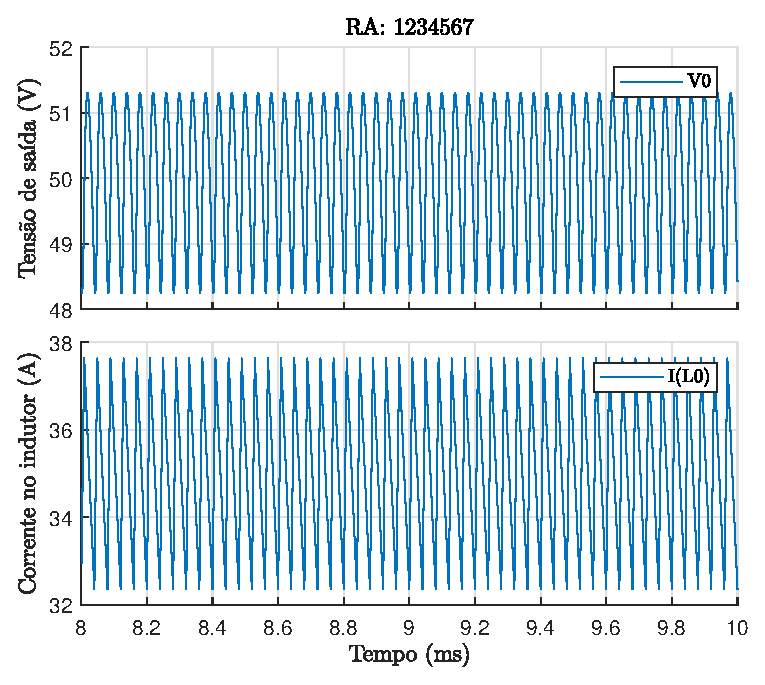
\includegraphics[width=1\linewidth]{Figs/Buck}
	\caption{Conversor Buck.}
	\label{fig:buck}
\end{figure}

\subsection{Parâmetros de projeto do conversor Buck}


A \tabref{tab:parametros} apresenta os parâmetros de projeto do conversor Buck.

% Tabela com parâmetros do conversor
% Tabela com parâmetros do conversor
\begin{table}[!ht]
\centering
\caption{Parâmetros de projeto do conversor Buck referente ao registro acadêmico de número $1234567$}
\label{tab:parametros}
\begin{tabular}{@{}ccc@{}}
\toprule
\textbf{Símbolo} & \textbf{Descrição} & \textbf{Valor}\\ \midrule
$f_s$ & Frequência de comutação & \SI{25}{\kilo\hertz}\\
$f_s$ & Frequência de amostragem & \SI{50}{\kilo\hertz}\\
$V_i$ & Tensão média de entrada  & \SI{225}{\V}\\
$V_0$ & Tensão média de saída  & \SI{50}{\V} \\
$P_0$ & Potência processada  & \SI{1750}{\W} \\
$R_0$ & Resistência de carga & \SI{1.4286}{\ohm} \\
$\Delta{i_{L_0}}$  & Ondulação de corrente & \SI{15}{\%}\\
$\Delta{v_{C_0}}$  & Ondulação de tensão & \SI{0.7}{\%}\\
$L_0$ & Indutância & \SI{296.2963}{\micro\henry}\\
$C_0$ & Capacitância & \SI{75}{\micro\farad}\\
\bottomrule
\end{tabular}
\end{table}






\section{Verificação do ponto de operação via simulação}

A análise teórica apresentada anteriormente deve ser verificada por simulação \cite{noauthor_psim_nodate}.

A \tabref{tab:steadystate} apresenta o ponto de operação do conversor Buck.

% Tabela com o ponto de operação do conversor
% Tabela com o ponto de opera��o do conversor
\begin{table}[!ht]
\centering
\caption{Ponto de opera��o do conversor Buck referente ao registro acad�mico de n�mero $1234567$}
\label{tab:steadystate}
\begin{tabular}{@{}ccc@{}}
\toprule
\textbf{S�mbolo} & \textbf{Descri��o} & \textbf{Valor}\\ \midrule
$G$ & Ganho est�tico & \SI{0.22222}{}\\
$D$ & Raz�o c�clida  & \SI{22.2222}{\%}\\
$I_0$ & Corrente m�dia na carga  & \SI{35}{\A} \\
$I_{L_0}$ & Corrente m�dia no indutor & \SI{35}{\A} \\
$V_C$ & Tens�o de controle  & \SI{0.22222}{\V} \\
$V_{CM}$ & Tens�o m�xima de controle  & \SI{1}{\V} \\
$V_{Cm}$ & Tens�o m�nima de controle  & \SI{0}{\V} \\
$R_a$ & Resist�ncia de medi��o & \SI{270}{\kilo\ohm} \\
$R_b$ & Resist�ncia de medi��o & \SI{1.2}{\kilo\ohm} \\
$H_v$ & Ganho de medi��o (tens�o) & \SI{4.4248}{\milli\V\per\V} \\
$R_s$ & Resist�ncia shunt & \SI{0.1}{\ohm} \\
$H_i$ & Ganho de medi��o (corrente) & \SI{0.1}{\A\per\A} \\
\bottomrule
\end{tabular}
\end{table}




\section{Verificação do modelo dinâmico via simulação}

\subsection{Função de transferência}

%\begin{equation}
%\frac{3317760000000001}{32768\,\left(s^2+\frac{1603454457173333\,s}{17179869184}+\frac{7549747199999989}{16777216}\right)}
%\end{equation}

\begin{figure}[!ht]
	\centering
	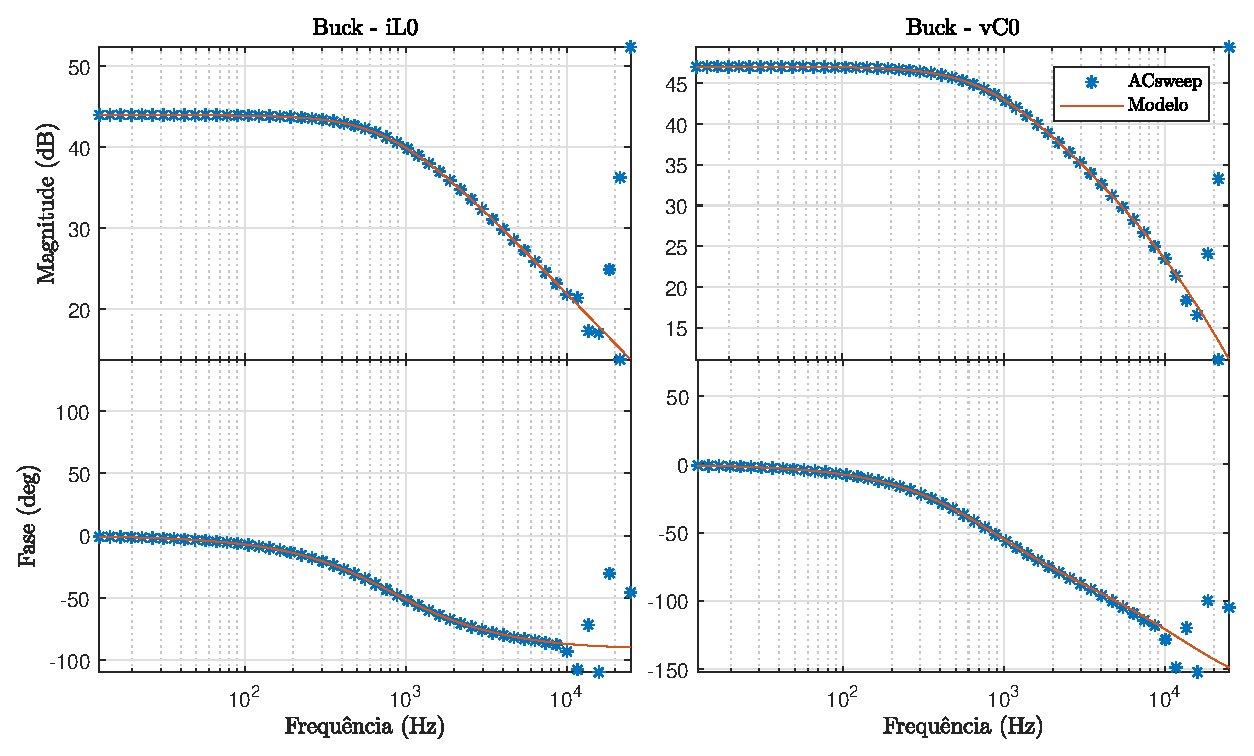
\includegraphics[width=1\linewidth]{Figs/Buck-ValidacaoModelo}
	\caption{Comparação do diagrama de Bode da função de transferência que relaciona uma variação da corrente na indutância em função da razão cíclica obtida via simulação no PSIM.}
	\label{fig:buck-il0}
\end{figure}


\section{Projeto do controlador de tensão}
Detalhes do projeto do controlador de tensão


\begin{figure}
	\centering
	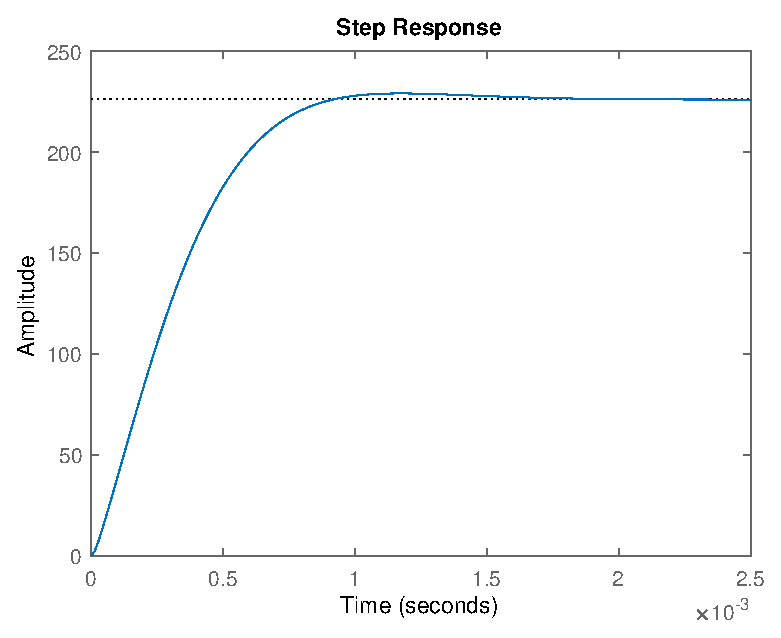
\includegraphics[width=0.8\linewidth]{Figs/StepResponse1malha}
	\caption{Resposta ao degrau de referência de tensão.}
	\label{fig:stepresponse1malha}
\end{figure}

% Tabela com a resposta ao degrau de referência
% Tabela com resposta ao degrau de referência
\begin{table}[!ht]
\centering
\caption{Resposta ao degrau de referência de tensão $v_{C0}$ do conversor Buck, registro acadêmico de número $1234567$}
\label{tab:resposta1malha}
\begin{tabular}{@{}cc@{}}
\toprule
\textbf{Descrição} & \textbf{Valor}\\ \midrule
Ganho proporcional & \SI{0}{}\\
Ganho integral & \SI{379.7032}{}\\
Tempo de subida & \SI{7.1922}{\milli\s}\\
Tempo de acomodação & \SI{7.4847}{\milli\s}\\
Tensão máxima de acomodação & \SI{225.8354}{\V}\\
Tensão mínima de acomodação & \SI{215.1245}{\V}\\
Sobresinal & \SI{0}{\V}\\
Tensão de pico & \SI{225.8354}{\V}\\
Tempo da tensão de pico & \SI{17.7167}{\milli\s}\\
\bottomrule
\end{tabular}
\end{table}




\section{Conclusões} 


As conclusões devem ser as mais claras possíveis, informando aos leitores sobre a importância do trabalho dentro do contexto em que se situa. As vantagens e desvantagens em relação aos já existentes na literatura devem ser comentadas, assim como os resultados obtidos e as possíveis aplicações práticas do trabalho.


\bibliographystyle{IEEEtran}

\bibliography{Refs/APS} % Inclui arquivos de referência

\balance


